\newpage
\chapter{Umsetzung}

\section{Übersicht}

Abbildung \ref{fig:component-overview} zeigt eine grobe Übersicht der wichtigsten Komponenten und deren Verbindungen untereinander. Dieses Design orientiert sich an der Kommunikationsarchitektur, die in Kapitel \ref{sec:communication-architecture} beschrieben wurde.

\begin{figure}[H]
	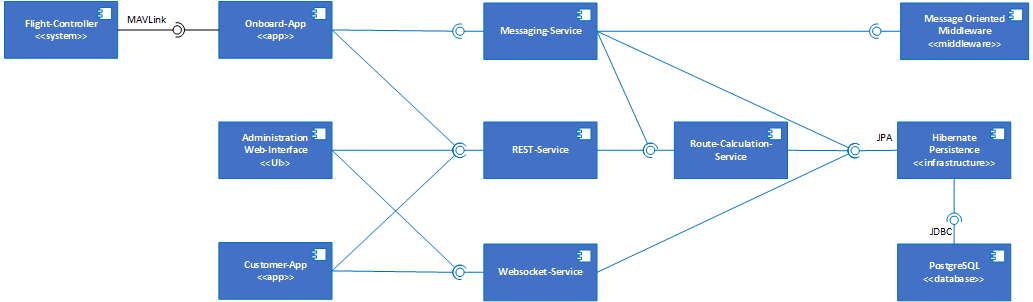
\includegraphics[width=1.0\textwidth]{images/component-overview.png}
	\caption{Übersicht wichtigsten Schnittstellen und deren Verbindungen }
	\label{fig:component-overview}
\end{figure}

\section{Implementierung}

\subsection{Messaging Provider}

Wie in der Architektur diskutiert, wurde, für die Kommunikation der Drohnen, für AMQP mit Messaging Broker entschieden.
Im folgenden werden einige Produkte verglichen: 
\subsubsection{Firebabse ( ehemals Google Cloud Messaging )}
Vorteile:
\begin{itemize}
	\item API ist gut dokumentiert
	\item Android wird unterstützt
\end{itemize} 
Nachteile:
\begin{itemize}
	\item Ist Kostenpflichtig ( ab 100 Verbindungen )
	\item Hat unterschiedliche Latenzen gemäss Erfrahungsbericht \ref{gcm-latenc}
\end{itemize}

\subsubsection{RabbitMQ}
Vorteile:
\begin{itemize}
	\item Ist opensource
	\item Kann Verbindung wiederherstellen bei Unterbrüchen
\end{itemize}

Nachteile:
\begin{itemize}
	\item Muss auf dem eigenen Server installiert werden
\end{itemize}

\subsubsection{ActiveMQ}
Vorteile:
\begin{itemize}
	\item Ist Open Source
\end{itemize}

Nachteile:
\begin{itemize}
	\item Kann nicht auf Android betrieben werden
\end{itemize}

\subsubsection{Entscheid}
Aufgrund unserer Anforderungen dass vom Android aus auf den Messaging Broker verbunden werden kann, und beim Verbindungsunterbrüche keine negativen Auswirkung haben sollten, kam nur RabbitMQ in Frage.

\subsection{Server}

\subsubsection{Play Framework}
Für den Server Teil wurde das Play Framework mit Java ausgewählt, denn grösstenteils mussten CRUD Operationen auf einer Weboberfläche dargestellt werden. Gründe die unsere Entscheidung untermauerten:

\begin{itemize}
    \item Fortschrittlicher O/R-Mapper im Framework integriert
    \item Vorgegebene MVC-Architektur (Speziell geeignet für CRUD-Operationen)
    \item Schnelle Implementation durch Spezialisierung auf diese Anwendungsart 
    \item Alle Entwickler des Projekts sind versiert in Java
    \item RabbitMQ Anbindung möglich
    \item WebSocket Anbindung möglich
\end{itemize}
An dieser Stelle sollte angemerkt werden, dass der De-Facto-Standard SpringMVC diese Liste ebenfalls vollständig abdeckt. Da wir bereits Erfahrungen mit SpringMVC gesammelt haben und Neugierig waren, ob die vielen guten Kommentare zu Play, auch in der Praxis berechtigt sind, entschieden wir uns zugunsten von Play.
\\
Während der Implementierung kristallisierten sich mehrere Schwächen des Frameworks heraus. 
Im Anhang \ref{ch:play_pitfalls} wird anhand einiger Beispiele erklärt, warum wir Play mit Java nur eingeschränkt weiterempfehlen können und welche Probleme damit aufgetreten sind.

\subsubsection{Kommunikation mit Drohnen}

Wie in der Architektur beschrieben, kommunizieren die Drohnen über AMQP mit dem Messaging-Broker. Um die Möglichkeit zu haben mit einzelnen Drohnen zu kommunizieren, müssen auf dem Server zur Laufzeit alle Verbindungen zu allen Drohnen bekannt sein. Ausserdem muss en möglich sein, eingehende Nachrichten an einem zentralen Punkt abzuarbeiten. Auf Grund der bestehenden MVC-Struktur der Play-Applikation haben wir uns entschieden, auch die Nachrichten aus dem Messaging-System in Controllern zu behandeln, wie es normalerweise nur mit HTTP-Requests geschieht.\\

Die Abbildung \ref{fig:drone-communication-diagram} zeigt ein Objekt-Diagramm von Instanzen, die die Kommunikation mit den Drohnen erlauben, sobald die Applikation gestartet ist.

\begin{figure}[H]
	\centering
	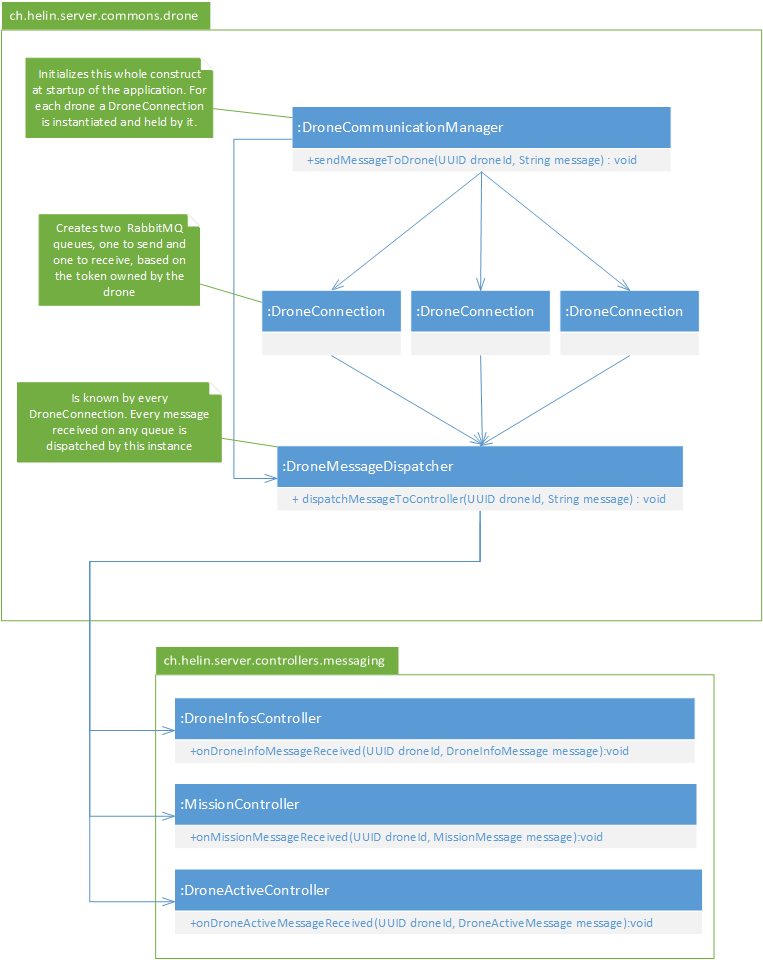
\includegraphics[width=0.8\paperwidth] {images/drone-communication-diagram.png}
	\caption{Objekt-Diagramm der Kommunkationsstruktur}
	\label{fig:drone-communication-diagram}
\end{figure}

\subsubsection{Verwendete Bibliotheken}

\begin{tabularx}{\textwidth}{|X|X|c|X|}
	\hline
	\textbf{Name} & \textbf{Verwendungszweck} & \textbf{Version} & \textbf{Lizenz} \\
	\hline \hline
	Hibernate ORM Mapper & objekt-relationales Mapping zwischen Datenbank und Models  & 5.1.0 & Apache 2.0\\
	\cmidrule{2-4}
	& \multicolumn{3}{l|}{\textbf{Begründung:} Hibernate ORM bietet die Erweiterung Hibernate Spatial, welcher als einziger OR-Mapper zu PostGIS Geometrie Objekten abbilden kann. }
	\\
	\hline 
	RabbitMQ Client & Client Komponente zur Kommunikation mit dem Rabbit MQ Broker & 3.6.0 &  Mozilla Public License 1.1, GPL 2, Apache 2.0 \\
	\hline 
	jGraphT & Graph Bibliothek für Java, um effizient Operationen auf dem Graph auszuführen & 0.9.2 &  LGPL, EPL \\
	\hline 
	Google GSON & JSON Serialisierungs / Deserialisierungs Bibliothek & 2.6.2 & Apache 2.0\\
	\hline 
\end{tabularx}

\subsection{Onboard-App}

\subsubsection{Entwicklungsumgebung}
Um den \Gls{Flight-Controller} mit \Gls{MAVLink} ansprechen zu können, musste eine Android/Java Library gefunden werden, die dies ermöglicht. Die Firma 3DR, der Hersteller des Pixhawk Flight-Controllers, stellt dafür eine Open-Source Android-API bereit. Die API konnte im App integriert werden erlaubt es, dem Flight-Controller direkt Befehle zu erteilen. Ausserdem kann man über diese Schnittstelle auch Telemetriedaten auslesen und Events handeln, z.B. Höhenänderungen. Damit war es möglich, die Drohne vom App und damit auch vom Server aus zu steuern.\\

Um während der Entwicklung laufend Tests durchzuführen, ohne jedes Mal mit der echten Drohne zu testen, verwendeten wir eine Software, die den Flight-Controller simuliert. Die Simulation verhält sich fast gleich wie ein richtiger Controller und hilft herauszufinden, ob die gesendeten Befehle die erwartete Wirkung erzeugen. Das erarbeiten der verschiedenen Setups war teilweise ziemlich aufwendig, je nachdem ob man neben der App noch eine Bodenstation an die Simulation anbinden wollte, die weitere Echtzeitinformationen liefert (siehe Abb. \ref{fig:test-setup-onboard}). Auf Github sind die verschiedenen Setups detailliert erklärt, um den Einstieg in die Entwicklung zu erleichtern.

\begin{figure}[H]
	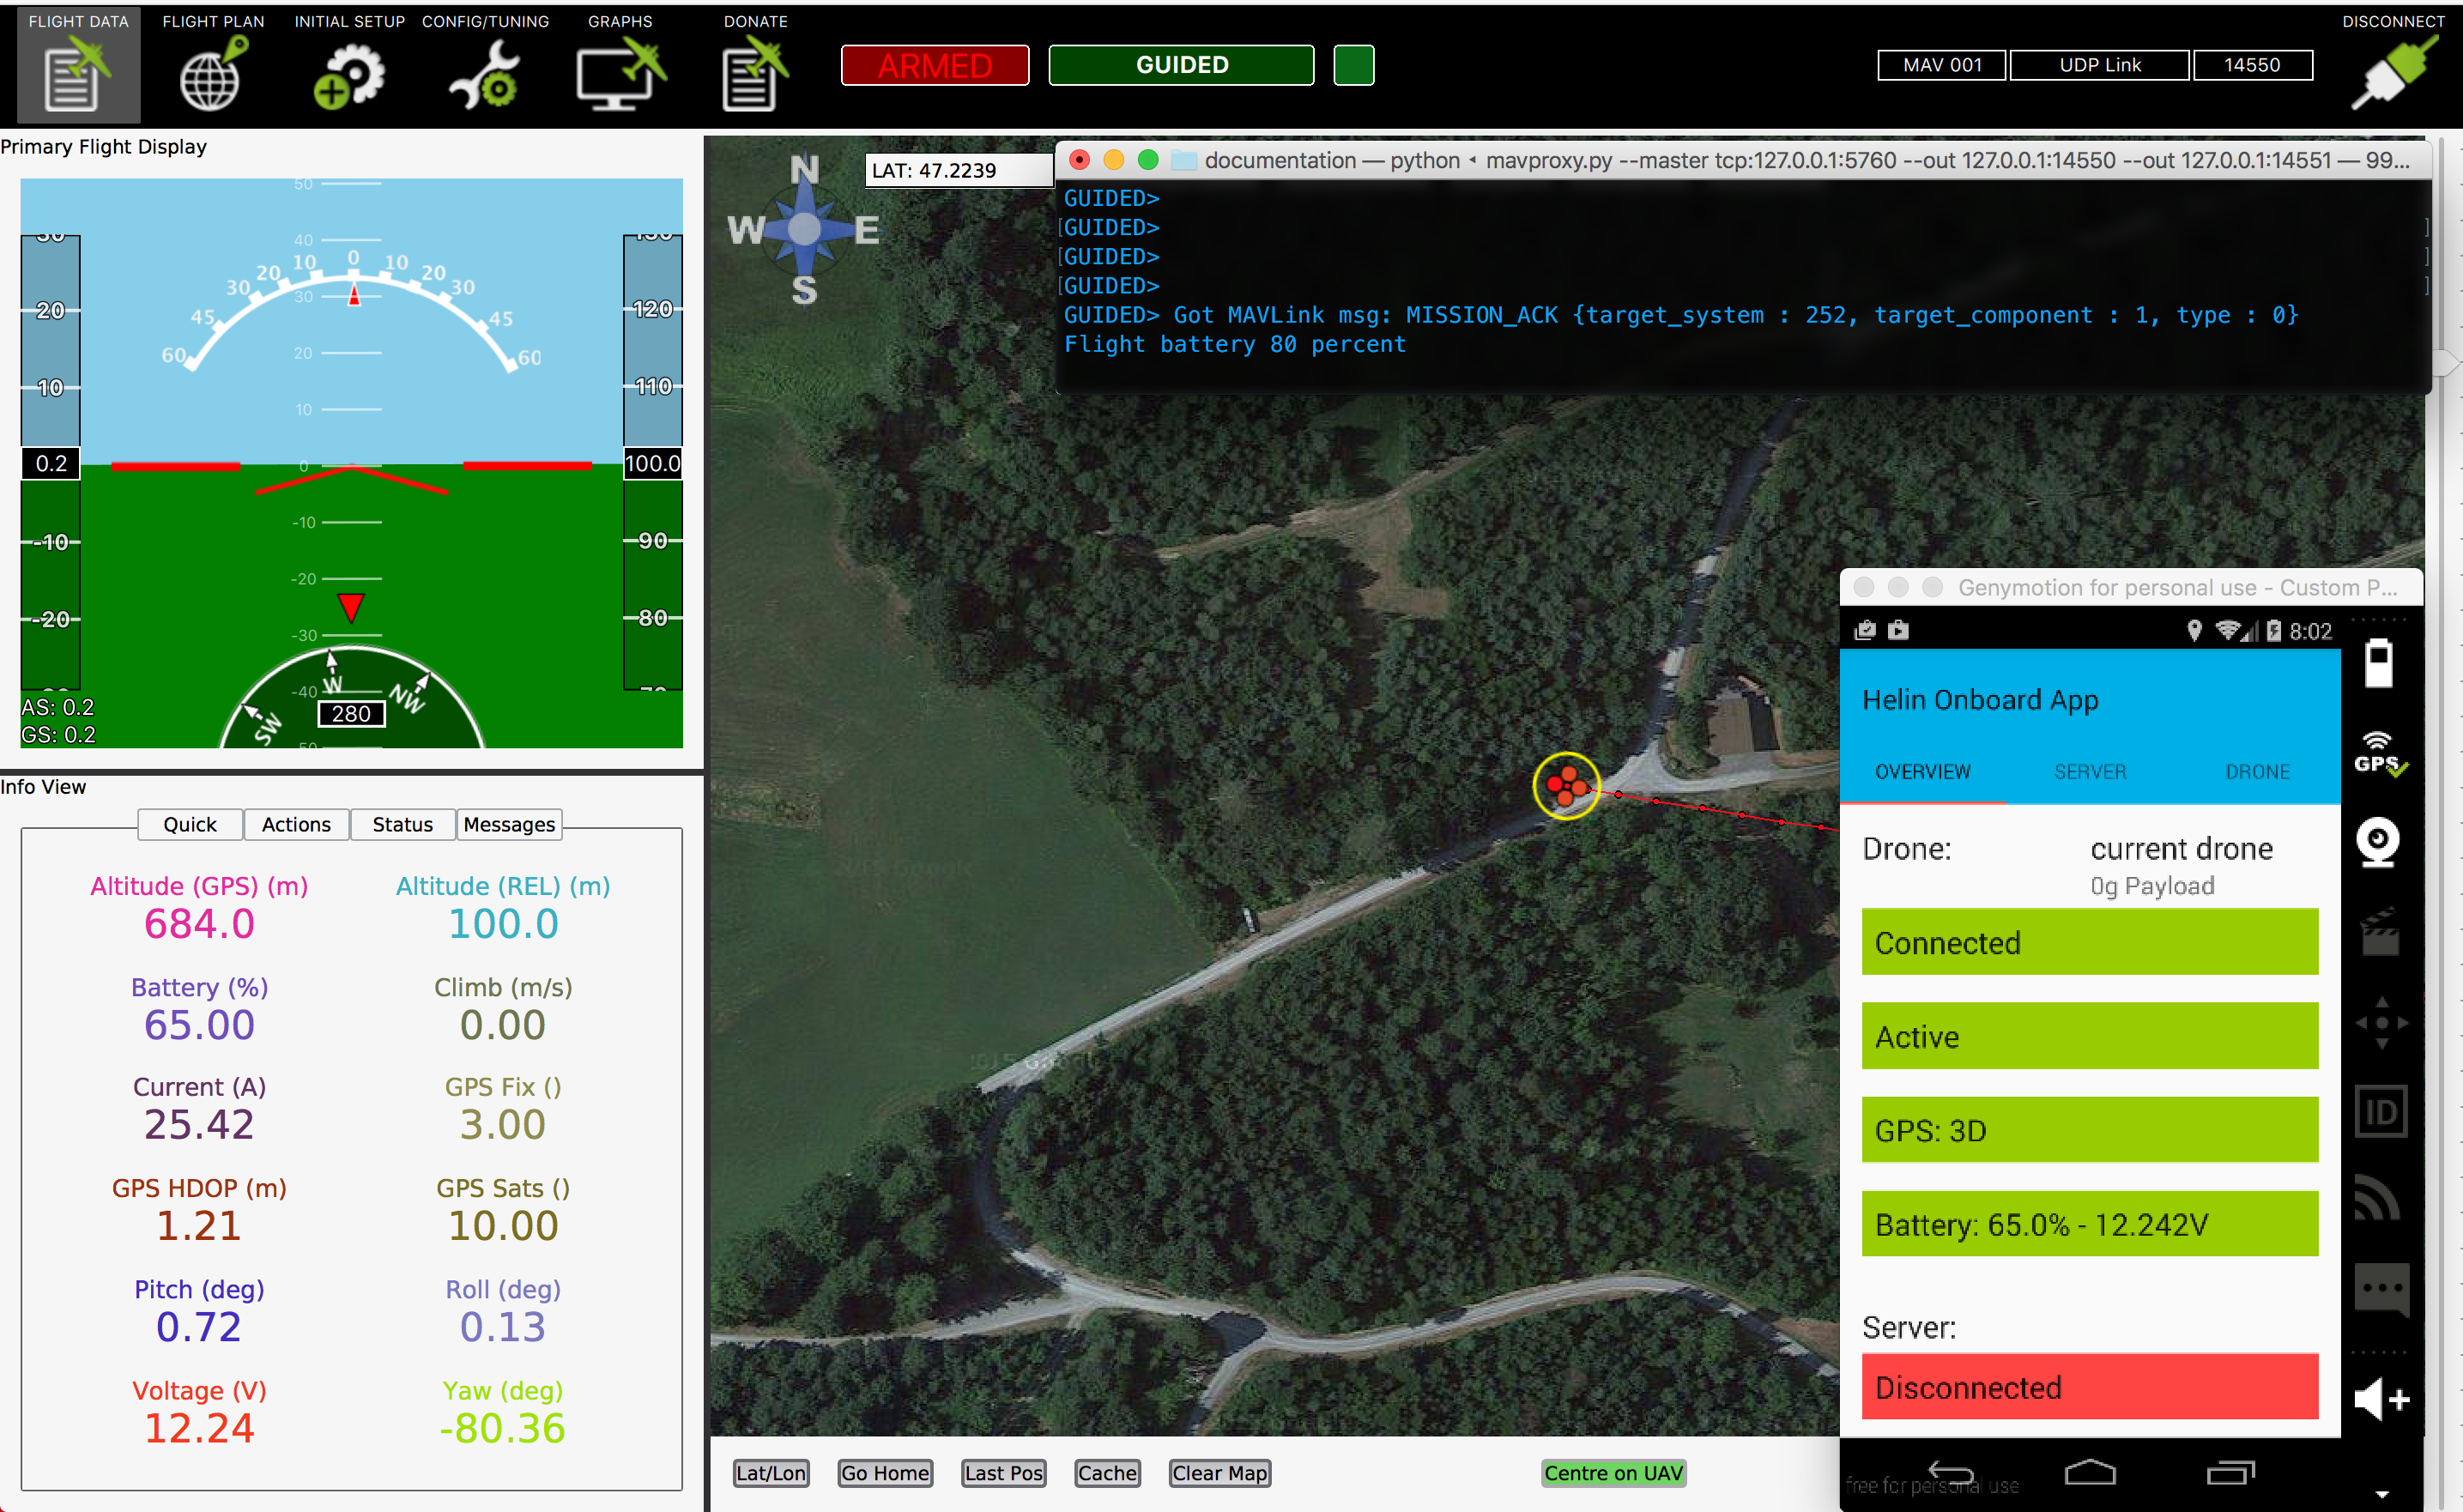
\includegraphics[width=1.0\textwidth]{images/test-setup-onboard.png}
	\caption{APM Planner 2.0 als Bodenstation und Android Emulator mit Onboard App}
	\label{fig:test-setup-onboard}
\end{figure}

\subsubsection{Verwendete Bibliotheken}
\begin{tabularx}{\textwidth}{|X|X|c|X|}
	\hline
	\textbf{Name} & \textbf{Verwendungszweck} & \textbf{Version} & \textbf{Lizenz} \\
	\hline \hline
	DroneKit-Android Client & Android API für MAV-Link Protokoll zum ansteuern der Drohne & 1.5.1 & Apache 2.0\\
	\hline 
	AMQP Messaging Library & Messaging für Android & 3.6.0 &  Mozilla Public License 1.1, GPL 2,  Apache 2.0 \\
	\hline 
	Lyra  & High availability Messaging & 0.4.3 &  Apache 2.0 \\
	\hline 
	Dagger  & Dependency Injection Framwork für Android & 2.0.1 &  Apache 2.0 \\
	\hline 
\end{tabularx}

\subsubsection{Kommunikation zum Server}

Die Kommunikation vom Onboard-App zum Server sollte bidirektional sein. 
Gemäss den nicht-funktionalen Anforderungen darf der Verbindungsabbruch keinen Einfluss auf die Mission haben.
Aufgrund der schlechten Erfahrung mit WebSocket auf mobilen Geräten und der ständigen Verbindungsabbrüche, kam diese nicht in Frage.
Eine alternative war Messaging. Wegen der zeitlichen Unabhängigkeit, vom Server und App, haben Verbindungsabbrüche keine schlimmen Konsequenzen.\\

Um bei Verbindungsabbrüchen die Mission nicht zu gefährden, wird die gesamte Mission vor dem Start übertragen, damit sie ausgeführt werden kann. Einzelne Wegpunke sind somit nicht auf eine stabile Internetverbindung angewiesen, da die Route bereits von Anfang bekannt ist. \\
Verbindungsabbrüche auf dem Mobiltelefon haben zweierlei Konsequenzen:	\\
\begin{itemize}
	\item{\textbf{Mobiltelefon kann die Messages vom Server nicht empfangen:} \\
		Dieses Szenario wird durch das RabbitMQ abgefangen. Der Messaging Broker cached die Nachrichten solange bis der Consumer (Mobiltelefon) wieder verfügbar ist. Es besteht somit kein zusätzlicher Handlungsbedarf auf dem Onboard-App.
	}
	\item{\textbf{Messages vom Mobiltelefon zum Server können nicht gesendet werden:} \\
		In diesem Fall kann der Übertragungsfehler nicht durch RabbitMQ abgefangen werden. Der Broker hat vom Producer (Mobiletelefon) noch keine Nachricht bekommen. Aus diesem Grund wird producerseitig eine Exception geworfen, die darauf hinweist, dass die Verbindung unterbrochen ist. In diesem Fall wird die Nachricht in einem Queue zwischengespeichert. Sämtliche Folgenachrichten, die während des Verbindungsunterbruchs nicht übertragen werden können, werden ebenfalls in dieser Queue gespeichert. Sobald die Verbindung wieder besteht, werden die Nachrichten aus der Queue gesendet.
	}
\end{itemize}
Mit diesen Massnahmen ist ein guter Kompromiss aus Zuverlässigkeit und Aufwand entstanden. Alle missionskritischen Nachrichten können übertragen werden. Telemetriedaten werden beim Verbindungsausfall verspätet übertragen
}


\subsubsection{Verbindungswiederherstellung}
Aus den nicht funktionalen Anforderungen ist zu entnehmen, dass bei einem Verbindungsunterbruch ein Reconnect stattfindet. Dieser Reconnect soll, sobald die Verbindung im GSM Netz wieder besteht nicht länger als 30s dauern. \\

Bei der Konfiguration von AMQP bestanden mehrere Möglichkeiten. Einersetis war der bekannte Backoff Algorithmus eine Option. Dieser Algorithmus arbeitet nach einem incrementellen Prinzip. Je länger der Unterbruch dauert, desto länger dauert es bis er die Verbindung wieder versucht aufzubauen. Auf der anderen Seite stand ein einfacher Interval-Algorithmus. Dieser versucht alle drei Sekunden die Verbindung wiederherzustellen, bis zum erfolgreichen Verbindungsaufbau. \\
Mit diesen Erkenntnissen haben wir folgende Messung gemacht:
\begin{table}
	\centering
	\begin{tabular}{|r|r|r|}
		\hline
		\textbf{Versuch} & \textbf{Backoff (s) } & \textbf{Interval 3s (s)} \\
		\hline
		1 & 17 & 7 \\
		2 &	7 & 7 \\
		3 & 9 & 7 \\
 		4 & 11 & 7 \\
		5 & 10 & 7 \\
		\hline
	\end{tabular}
	\caption{Anzahl Sekunden für den Reconnect nach jedem Versuch}
\end{table}
Aus diesen Erkenntnissen standen beide Möglichkeiten offen, denn beide erfüllen die Anforderungen und haben somit auch keine Auswirkungen auf die Qualität. Am Ende wurde bewusst auf den BackOff Algorithmus gesetzt. Der Backoff Algorithmus benötigt zwar deutlich länger für einen Reconnect als das fixe Zeitinterval. Die hetrogene Verteilung der Wiederverbindungszeiten spricht aber für den Backoff Algorithmus. Sollte es zu Probleme auf der Serverseite kommen, so werden nicht alle Geräte gleichzeitig einen Reconnect probieren - der Reconnect passiert somit gestaffelt. Dies bringt zusätzlich Stabilität ins System.

\subsubsection{Android Process Lifecycle} 
Da die OnboardApp auf einem Android Betriebssystem läuft, mussten gewisse Voraussetzungen geprüft werden. Im Grund kann davon ausgegangen werden, dass die Applikation immer im Vordergrund steht. Es ist doch sehr unwahrscheinlich, dass die Appliaktion in den Hintergrund rückt, weil eine andere Applikation verwendet wird. \\
Laut Android Dokumentation ist das Verhalten einer Applikation im Hintergrund nicht deterministisch \cite{androidGuide}. Sollte eine Applikation im Hintergrund gewisse Garantien haben, so muss von einem Service und der spezifischen Implementierung eines Services gesprochen werden. Im Fall der OnboardApp und den getroffenen Annahmen, wurde davon abgesehen, da die Applikation während des Fluges nicht gewechselt wird.\\


\subsection{Customer App}
Gemäss Aufgabenstellung sollte ein Prototyp für eine App, mit welchem Bestellungen am System abgegeben können, entwickelt werden.
Diese App wurde als letzte Komponente entwickelt, da sie erst getestet werden konnte als die Server- und Onboard-App-Komponenten fertiggestellt waren.

Um manuelle Tests der Bestell-API möglich zu machen, wurde in der Administrations-Seite eine "'Fake Order"' Funktionen eingeführt. 
Diese imitiert eine Bestellung des Kunden und schickt eine Anfrage mit vordefinierten Koordinaten und Produkten an das System.

\begin{figure}[H]
	\centering
	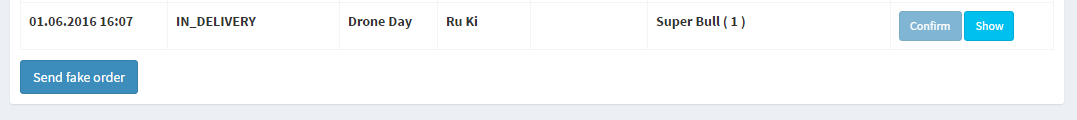
\includegraphics[width=1\textwidth] {images/customer-app-fake-order.png}
	\caption{Send Fake Order within Administrator Page}
\end{figure}

Anders als die Onboard-App, welche native mit Java entwickelt wurde und nur auf Android läuft, entschieden wir uns beim Bestell-App für eine Cross-Plattform Lösung, welche Android und iOS unterstützt. \\

Auch wenn gemäss der Aufgabenstellung keine iOS App gefordert war, stellte sich doch die Frage ob man die iPhone-Kunden ausschliessen soll und spätere Entwickler zwingt, einen grossen Teil des Codes in einer nativen iOS App duplizieren zu müssen. Mit einem Marktanteil von 42.2\% (Zahlen 2015) \cite{ios-user} von iOS Benutzern in der Schweiz, ist anzunehmen, dass zu einem späteren Zeitpunkt eine iPhone App implementiert werden muss.\\

Deshalb wurde auf Xamarin Forms gesetzt, welches ermöglicht, die ganzen Service-Klassen und einen Teil der Benutzeroberfläche für die verschiedenen Plattformen nur einmal zu implementieren.

Die App wurde in einer minimalen Ausbaustufe erstellt, erfüllt aber bereits alle nötigen Funktionalen Anforderungen. In Abbildung \ref{fig:customer-app-flow} wird gezeigt, wie ein Benutzer durch die App navigieren kann. 

Besonders wichtig ist die Anzeige des berechneten Abwurfpunktes vor der Bezahlung der Ware, sowie die Anzeige der Drohnenposition während des Anflugs.  

\begin{landscape}
	\begin{figure}[h]
		\centering
		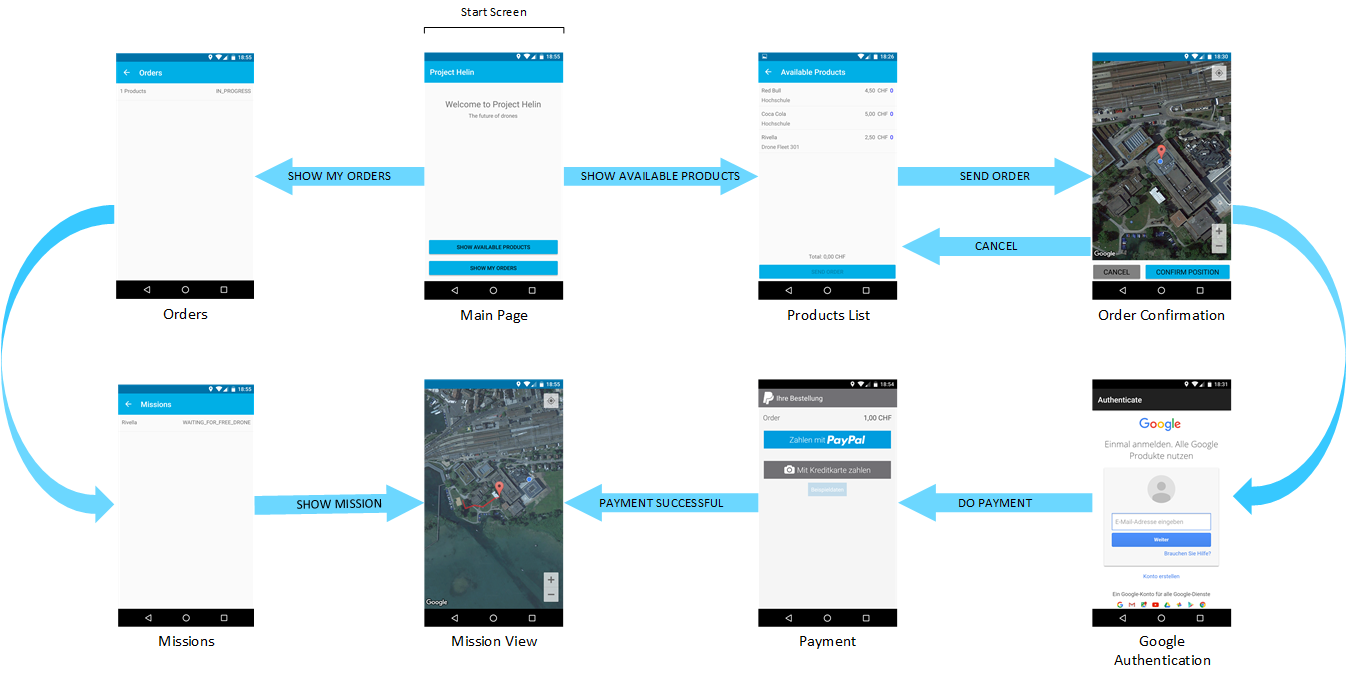
\includegraphics[width=0.8\paperheight] {images/customer-app-pages.png}
		\caption{Übersicht der Customer App mit allen Verknüpfungen zwischen den Screens}
		\label{fig:customer-app-flow}
	\end{figure}
\end{landscape}

\subsubsection{Verwendete Bibliotheken}
\begin{tabularx}{\textwidth}{|X|X|c|X|}
	\hline
	\textbf{Name} & \textbf{Verwendungszweck} & \textbf{Version} & \textbf{Lizenz} \\
	\hline \hline
	Paypal Forms & Paypal integration für Xamarin.Forms & 2.0.4 & MIT \\
	\hline 
	Xamarin Forms & Plattform übergreifende Komponente für Xamarin & 2.2.0.45 & \url{https://www.xamarin.com/license} \\
	\hline 
	Websocket.PCL & Plattformübergreifende WebSocket Anbindung & 1.1.9 & MIT \\
	\hline 
	Newton.Json & Json zu Object mapper & 8.0.3 & MIT \\
	\hline 
\end{tabularx}

\subsection{Sicherheit}
Es ist essentiell, dass die Sicherheit bei der Kommunkation zwischen Server und Drohne gewährleistet ist, da sonst die Kontrolle über eine Drohne übernommen werden könnte (siehe auch NFRs). Um diese Sicherheit zu gewährleisten wurde ein Prozess eingeführt, der es ermöglicht die Zugangsdaten für den RabbitMQ-Broker und die Queue-Namen geheim zu halten: \\

Die Onboard-App registriert sich über einen HTTPS Request beim Server. Bei erfolgreicher Registrierung der Drohne, wird ein Token sowie der Benutzer und das Kennwort für die Verbindung zu RabbitMQ an die Onboard-App geschickt. Mit diesen Informationen kann sich die App mit dem Messaging Broker über eine verschlüsselte Leitung verbinden.\\

Für die darauf folgende Kommunikation mit dem Broker, werden mit Hilfe des Tokens zwei Queues erzeugt: 
\begin{itemize}
	\item \{token\}-Drone-To-Server
	\item  \{token\}-Server-To-Drone
\end{itemize}

Über diese Queues können jetzt Nachrichten ausgetauscht werden. \\

Ein Angreifer müsste mit dieser Methode den Token herausfinden und auch die Zugangsdaten für den Broker kennen, um mit einer Drohne zu kommunizieren. Falls jemand es aber doch schaffen würde, die Benutzerdaten auszulesen, gibt es trotzdem noch $2^{122}$ mögliche Tokens, die durchprobiert werden müssten. \\

\section{Projektgrösse}

Folgende Statistiken wurden am Ende der Arbeit erstellt um einen Eindruck der Grösse des Projekts zu erhalten.\\

\begin{figure}[H]
	\centering
	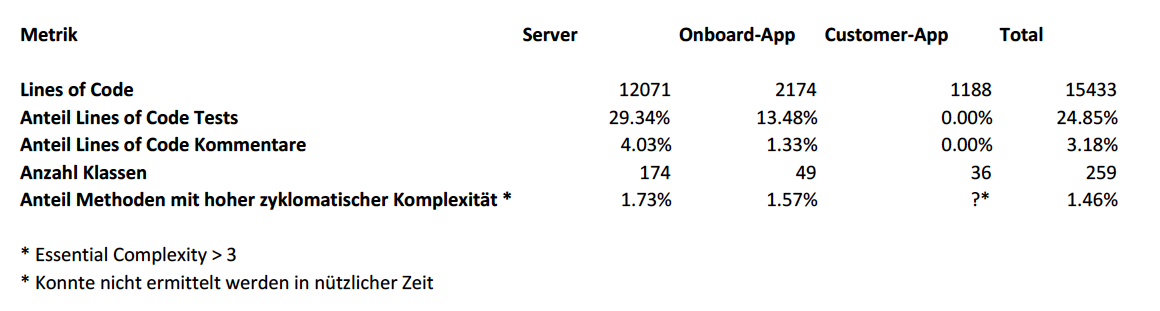
\includegraphics[width=1.0\textwidth] {images/code-metrics.png}
	\caption{Code Metriken nach Abschluss der Arbeit}
	\label{fig:code-metrics}
\end{figure}

In Abbildung \ref{fig:code-metrics} sind vor allem der geringe Anteil von Methoden mit hoher essentieller Komplexität\cite[S. 79]{MCCABE} hervorzuheben. Alle Methoden mit hoher Komplexität wurden vom Team geprüft, konnten aber nicht mehr verbessert werden. Hauptsächlich sind dies 'equals' Methoden von grösseren DTOs oder es handelt sich um MessageConverter, die einfach alle verschiedenen Messagetypen verschieden behandeln müssen. Das folgende Beispiel zeigt die Methode mit der höchsten zyklomatischen Komplexität der Server-Applikation (Essentielle Komplexität = 10, Cyclomatische Komplexität = 10). \\


\begin{lstlisting}
private Message parseMessageWithoutCare(String messageAsJson) {
	...
	switch (payloadType) {
		case ConfirmCargoLoaded:
			return gson.fromJson(messageAsJson, ConfirmCargoLoaded.class);
		case NotifyCargoDrop:
			return gson.fromJson(messageAsJson, NotifyCargoDrop.class);
		case DroneInfo:
			return gson.fromJson(messageAsJson, DroneInfoMessage.class);
		case DroneDto:
			return gson.fromJson(messageAsJson, DroneDtoMessage.class);
		case AssignMission:
			return gson.fromJson(messageAsJson, AssignMissionMessage.class);
		case FinalAssignMission:
			return gson.fromJson(messageAsJson, FinalAssignMissionMessage.class);
		case ConfirmMission:
			return gson.fromJson(messageAsJson, ConfirmMissionMessage.class);
		case FinishedMission:
			return gson.fromJson(messageAsJson, FinishedMissionMessage.class);
		case DroneActiveState:
			return gson.fromJson(messageAsJson, DroneActiveStateMessage.class);
	}
}

\end{lstlisting}

Da diese Methode gut strukturiert ist und auch gut verstanden werden kann, gibt es keinen Grund, diese auf Grund der Metrik anzupassen.

\section{Qualitätssicherung}

\label{quality-assurance}

\subsection{Prozesse}

Zur Qualitätssicherung wurde im Projektmanagement-Tool neben Todo, In Progress und Done ein neuer Quality-Assurance-Status für die Issues eingeführt. Alle Issues in diesem Status mussten von einem anderen Teammitglied überprüft werden, bevor sie auf Done geschoben werden konnten. \\

Die Überprüfung eines Issues beinhaltet folgende Aufgaben:

\begin{itemize}
	\item{Akzeptanzkriterien aus der User-Story manuell prüfen}
	\item{Code-Review durchführen (Intensität je nach Grösse und Komplexität des geschriebenen Codes)}
	\item{Code auf Vertösse gegen Style-Guide prüfen}
	\item{Prüfen der Tests vorhanden sind}
\end{itemize}

Damit konnten viele Fehler früh entdeckt werden und die Code-Qualität konnte über die ganze Projektdauer konstant gehalten werden.

\subsection{Continous Integration}

Als Build-Server haben wir TeamCity verwendet. Dort waren alle Projekte (ausser Customer-App) jeweils mit einem Build für den develop- und master-branch eingerichtet. Alle Builds führten die nötigen Tests aus und produzierten ein entsprechendes Artifact für das Deployment. Das Deployment für den Server wurde ebenfalls automatisiert.

\subsection{Testing}

Je nach Plattform wurden andere Formen von Tests durchgeführt:

\subsubsection{Server}
\begin{figure}[h]
	\centering
	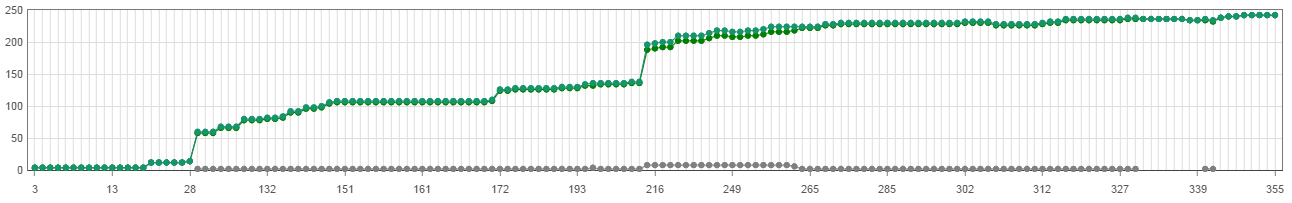
\includegraphics[width=1\textwidth] {images/test-count-chart.png}
	\caption{Anzahl Tests über die Zeit. Grün (erfolgreiche Tests) und Grau ( ausgeschlossene )}
\end{figure}

Auf dem Server wurden vor allem E2E- und Integration-Tests verwendet um die Funktionalität zu prüfen. Wir haben uns bei den meisten Kompoonenten bewusst gegen Unit-Tests entschieden, da auf dem Server nur wenig Logik zu finden ist, die nicht von der Datenbank oder der RabbitMQ-Connection abhängt. Unit-Tests hätten deswegen nur einen ganz kleinen Teil der Anwendungen abdecken können und wären in den meisten Fällen sehr aufwendig gewesen. Bei der Routenberechnung hingegen konnte sehr gut mit Unit-Tests gearbeitet werden.\\

Wir haben darauf geachtet, dass immer nur die minimale Integrationsstufe gewählt wurde. Für die Simulation eines Benutzers (E2E) wurde Selenium verwendet, das wiederum einen Firefox Browser verwendet. Für die Api- und Messaging-Controller wurden Integrationtests verwendet, welche keinen Browser benötigen.\\

Es wurde eine \textbf{durchschnittliche Testabdeckung von 72\%} über das ganze Projekt erreicht. In wichtigen Packages liegt diese aber meist über 85\%.

\subsubsection{Onboard-App}

Beim Onboard App wurden nur Unit-Tests ausgeführt. Der Aufbau von E2E Tests ist denkbar, hätte den Rahmen dieser Arbeit aber gesprengt. Deshalb wurden hauptsächlich die Message-Handler und die Daten-Mapper getestet. Diese haben eine \textbf{Testabdeckung von 86\%}.

\subsubsection{Customer-App}

Bei der Customer App wurden keine Tests eingerichtet, da es sich um einen Prototyp handelt.


